\documentclass[unicode,10pt,a4paper,oneside,numbers=endperiod,openany]{scrartcl}
\usepackage{tikz}
\usepackage{pgfplots}
\usepgfplotslibrary{colorbrewer} % better colors
\pgfplotsset{compat=1.18}
\input{assignment.sty}
\usepackage{amsmath}
\usepackage{url}
\usepackage{xcolor}
\usepackage{subcaption}
\usepackage{listings}
\usepackage{multirow}
\lstdefinestyle{grayverbatim}{
  basicstyle=\ttfamily,%
  backgroundcolor=\color{gray!10},%
  frame=single,%
  framesep=3pt,%
  breaklines=true,%
  columns=fullflexible%
}
\definecolor{lightbluehighlight}{RGB}{204,232,255}

\begin{document}


\setassignment
\setduedate{Monday 07 April 2025, 18:00 CEST}

\serieheader{High-Performance Computing Lab for CSE}{2025}
            {Student: Riccardo Polo}
            {Discussed with:}
            {Solution for Project 3}{}
\newline

\assignmentpolicy

\newpage
\section{Task: Implementing the linear algebra functions and the stencil
         operators [50 Points]}
\subsection{Numerical method }
We consider Fisher's reaction--diffusion equation on the square domain \(\Omega=[0,1]^2\), where the population concentration \(s(x,y,t)\) evolves under the combined effects of diffusion and logistic growth (eq. \ref{eq:fisher}).
\begin{equation}
\label{eq:fisher}
\frac{\partial s}{\partial t} = D \biggl(\frac{\partial^2\, s}{\partial x^2} + \frac{\partial^2\, s}{\partial y^2}\biggr) s + R s (1 - s)
\end{equation}
The problem is complemented by constant Dirichlet boundary conditions \(s=0.1\) on \(\partial\Omega\) and by an initial condition consisting of a localized perturbation, with \(s=0.2\) inside a small disk centered at \((1/4,1/4)\) and \(s=0.1\) elsewhere.

The spatial domain is discretized on a uniform Cartesian grid with \((n+2)\times(n+2)\) points, where only the \(n^2\) interior values are treated as unknowns. Spatial derivatives are approximated by a second-order central finite-difference scheme, yielding the standard five-point stencil, while time integration is performed using the implicit Euler method. At each time step, this results in a nonlinear algebraic system for the updated concentration field \(s^k\).

The nonlinear system is solved with Newton's method applied to the residual equation \(f(s^k)=0\). At each Newton iteration, the corresponding linearized correction problem involving the Jacobian of the residual is solved approximately with a matrix-free Conjugate Gradient method, thereby avoiding explicit Jacobian inversion. The converged solution at time step \(k\) is then used as the initial guess for the subsequent time step.\\

We were asked to implement the linear algebra functions and the stencil operators, which are used in the Conjugate Gradient method and in the Newton's method, respectively.\\
One can look at the linear algebra functions in the file \texttt{linalg.cpp} and the stencil operators in the file \texttt{operators.cpp}.\\
In particular for the stencil operators we have to implement the residual function $f_{(i,j)}^k$ for the interior points, and for the points on the boundaries.\\
The residual function in the interior points is given by eq. 7 of the project handout. For the boundery points, we have to take into account the Dirichlet boundary conditions, obtaining:
\begin{align*}
    \text{East: }\quad &f_{(n+1,j)}^k = -(4+\alpha) s_{(n+1,j)}^k + s_{(n,j)}^k + 0.1 + s_{(n+1,j-1)}^k + s_{(n+1,j+1)}^k + \beta{s_{(n+1,j)}^k}(1-s_{(n+1,j)}^k) + \alpha s_{(n+1,j)}^{k-1}\\
    \text{West: }\quad &f_{(0,j)}^k = -(4+\alpha) s_{(0,j)}^k + 0.1 + s_{(1,j)}^k + s_{(0,j-1)}^k + s_{(0,j+1)}^k + \beta{s_{(0,j)}^k}(1-s_{(0,j)}^k) + \alpha s_{(0,j)}^{k-1}\\
    \text{North: }\quad &f_{(i,n+1)}^k = -(4+\alpha) s_{(i,n+1)}^k + s_{(i-1,n+1)}^k + s_{(i+1,n+1)}^k + 0.1 + s_{(i,n)}^k + \beta{s_{(i,n+1)}^k}(1-s_{(i,n+1)}^k) + \alpha s_{(i,n+1)}^{k-1}\\
    \text{South: }\quad &f_{(i,0)}^k = -(4+\alpha) s_{(i,0)}^k + s_{(i,1)}^k + 0.1 + s_{(i-1,0)}^k + s_{(i+1,0)}^k + \beta{s_{(i,0)}^k}(1-s_{(i,0)}^k) + \alpha s_{(i,0)}^{k-1}\\
    \text{NE corner: }\quad &f_{(n+1,n+1)}^k = -(4+\alpha) s_{(n+1,n+1)}^k + s_{(n,n+1)}^k + 0.1 + s_{(n+1,n)}^k + \beta{s_{(n+1,n+1)}^k}(1-s_{(n+1,n+1)}^k) + \alpha s_{(n+1,n+1)}^{k-1}\\
    \text{NW corner: }\quad &f_{(0,n+1)}^k = -(4+\alpha) s_{(0,n+1)}^k + 0.1 + s_{(1,n+1)}^k + s_{(0,n)}^k + \beta{s_{(0,n+1)}^k}(1-s_{(0,n+1)}^k) + \alpha s_{(0,n+1)}^{k-1}\\
    \text{SE corner: }\quad &f_{(n+1,0)}^k = -(4+\alpha) s_{(n+1,0)}^k + s_{(n,0)}^k + 0.1 + s_{(n+1,1)}^k + \beta{s_{(n+1,0)}^k}(1-s_{(n+1,0)}^k) + \alpha s_{(n+1,0)}^{k-1}\\
    \text{SW corner: }\quad &f_{(0,0)}^k = -(4+\alpha) s_{(0,0)}^k + 0.1 + s_{(1,0)}^k + s_{(0,1)}^k + \beta{s_{(0,0)}^k}(1-s_{(0,0)}^k) + \alpha s_{(0,0)}^{k-1}
\end{align*}

The \texttt{main.cpp} implements the time integration of the nonlinear system arising from the implicit discretization of Fisher's equation.\\
For each time step $k$, Newton's method is applied to solve the nonlinear system \(f(s^k)=0\). At iteration \(m\), the residual is computed as:
\[
r^{(m)} = f\bigl(s^{k,m}\bigr),
\]
which corresponds to the call to the stencil operator \texttt{diffusion}. The convergence of the nonlinear iteration is monitored through the Euclidean norm of the residual:
\[
\|r^{(m)}\|_2.
\]
If the residual falls below a prescribed tolerance, the Newton iteration is terminated.\\
Otherwise, the Newton correction \(\delta s^{(m)}\) is obtained by approximately solving the linearized system
\[
J\bigl(s^{k,m}\bigr)\,\delta s^{(m)} = r^{(m)},
\]
where \(J\) denotes the Jacobian of the residual. This system is solved using a matrix-free Conjugate Gradient method, implemented in \texttt{hpc\_cg}, which avoids the explicit construction of the Jacobian matrix.

If the CG solver converges, the solution is updated according to the Newton step:
\[
s^{k,m+1} = s^{k,m} - \delta s^{(m)},
\]
implemented via the BLAS-like operation \texttt{hpc\_axpy}.

The process is repeated until either convergence is reached or a maximum number of Newton iterations is exceeded. If convergence is not achieved, the simulation is terminated and an error message is reported.
\subsection{Results}
The implementation of the linear algebra functions and the stencil operators was successful, as the program runs without errors and produces results consistent with the expected behavior of the solution to Fisher's equation.\\
In particular the output is given by the following listing
\begin{lstlisting}[style=grayverbatim]
================================================================================
                      Welcome to mini-stencil!
version   :: C++ Serial
mesh      :: 128 * 128 dx = 0.00787402
time      :: 100 time steps from 0 .. 0.005
iteration :: CG 300, Newton 50, tolerance 1e-06
================================================================================
simulation took 0.157575 seconds
1513 conjugate gradient iterations, at rate of 9601.76 iters/second
300 Newton iterations
--------------------------------------------------------------------------------
### 1, 128, 100, 1513, 300, 0.157575 
\end{lstlisting}
Looking at the project handout and comparing with our results, we can see that the number of CG iterations and Newton iterations are consistent with the expected values, which indicates that our implementation is correct.\\
We can also see in figures \ref{fig:initial} and \ref{fig:final} the initial and final solution of the problem, which are consistent with the images provided in the project handout, confirming the correctness of our implementation.
\begin{figure}[htbp]
    \centering
    \begin{subfigure}{0.5\textwidth}
        \centering
        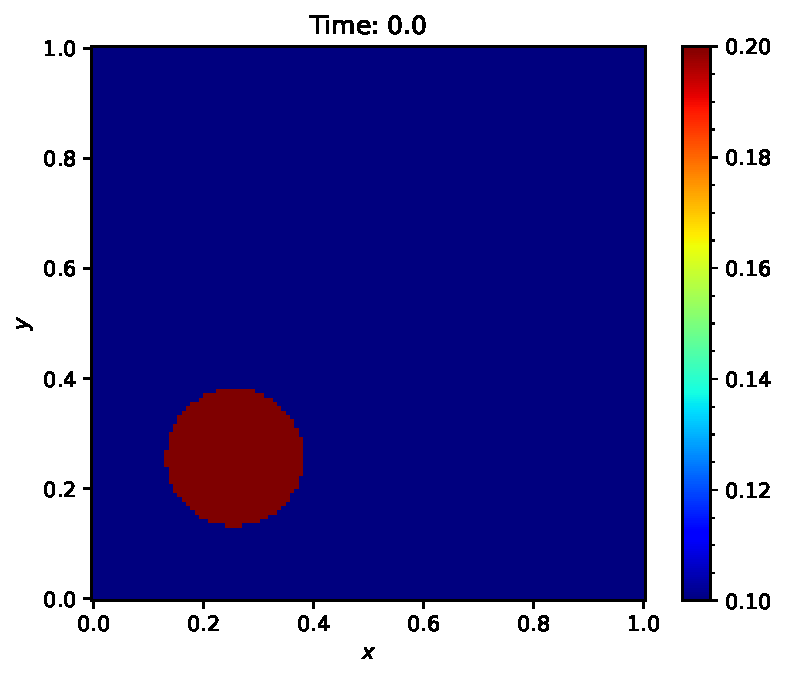
\includegraphics[width=\textwidth]{../01_serial/output_initial.pdf}
        \caption{Initial solution}
        \label{fig:initial}
    \end{subfigure}%
    \begin{subfigure}{0.5\textwidth}
        \centering
        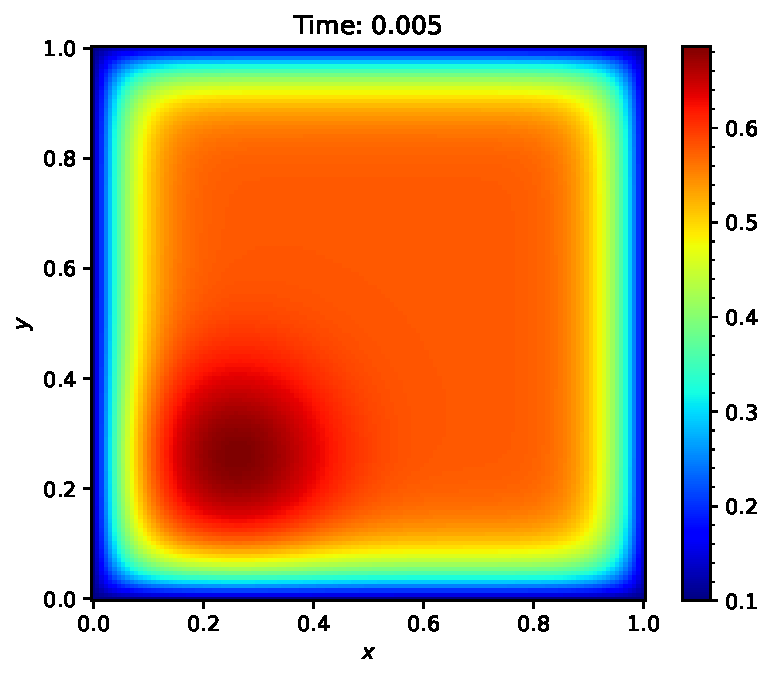
\includegraphics[width=\textwidth]{../01_serial/output_final.pdf}
        \caption{Final solution}
        \label{fig:final}
    \end{subfigure}
    \caption{Comparison between initial and final solution}
    \label{fig:solution}
\end{figure}

\newpage
\section{Task: Adding OpenMP to the nonlinear PDE mini-app [50 Points]}

\end{document}
